\documentclass[11pt]{article}
\usepackage{amsmath, amssymb, amsthm}

\usepackage{fancyhdr}

\usepackage{tikz}

%Listings stuff
\usepackage{listings}
\usepackage{lstautogobble}
\usepackage{color}

\definecolor{gray}{rgb}{0.5,0.5,0.5}
\lstset{
basicstyle={\small\ttfamily},
tabsize=3,
numbers=left,
numbersep=5pt,
numberstyle=\tiny\color{gray},
stepnumber=2,
breaklines=true
}

%Format stuff
\pagestyle{fancy}
\headheight 35pt

%Header info
\chead{\Large \textbf{Dijkstra's Algorithm}}
\lhead{}
\rhead{}

\begin{document}
	Dijkstra's algorithm computes the shortest path to all other vertices in a directed graph from a given source vertex, given that each edge has a non-negative length.
	
\section{Algorithm}
	\begin{lstlisting}[autogobble=true,mathescape]
		def Dijkstra(G, s):
			for x in V:
				d[x] = $\infty$
				p[x] = None
			d[s] = 0
			Q = V
			
			while Q not empty:
				Pick x in Q to minimize d[x]
				Q -= {x}
				
				for (x, y) in E:
					if d[x] + w(x, y) < d[y]:
						d[y] = d[x] + w(x, y)
						p[y] = *x
						
			return d, p
	\end{lstlisting}

	All shortest path lengths are in \verb|d| when the algorithm finishes, and \verb|p| contains a pointer to the parent vertex in the shortest path for each vertex. To get the shortest path to \verb|v| as a series of vertices, run a DFS on \verb|p| starting at \verb|p[v]| and reverse the result. 

\section{Analysis}
	If \verb|d| is kept as a standard array, then the algorithm runs in $\Theta(n^2)$ (obvious). However, the way \verb|d| is used in the algorithm naturally lends itself to a min-heap representation. If we use a min-heap for \verb|d|, then the runtime for the algorithm is
	\begin{equation}
		\Theta(n\lg n + \sum_{x\in V} |\text{adj}(x)| \lg n)
	\end{equation}
	Because $\sum |\text{adj}(x)| \leq |E|$, the expression simplifies to $\Theta(n\lg n + m\lg n)$, which for a dense graph ($m >> n$) is $\Theta(m\lg n)$.
	
\section{Proof}
	To illustrate the concept behind the proof, imagine $G$ as a radial graph:
	
	\begin{center}
	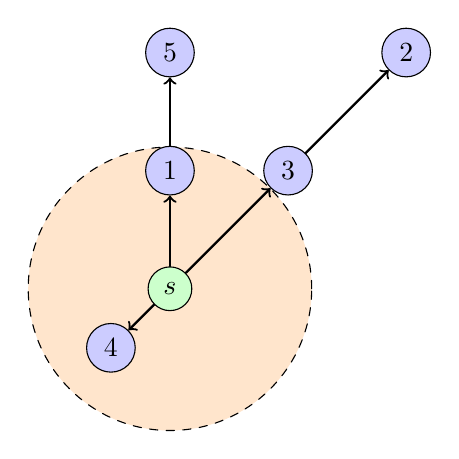
\begin{tikzpicture}
		[scale=1.5,line cap=round,
		%Styles
		axes/.style=,
		important line/.style={very thick},
		information text/.style={rounded corners,fill=red!10,inner sep=1ex},
		dot/.style={circle,inner sep=1pt,fill,label={#1},name=#1},
		main node/.style={circle,fill=blue!20,draw}			
		]
		
		%Colors
		\colorlet{anglecolor}{green!50!black}	%angle arcs/lines
		
		%The graphic
		\filldraw[dashed,fill=orange!20] (0, 0) circle (1.2cm);
		\node[circle,fill=green!20,draw] (s) at (0, 0) {$s$};
		\node[main node] (1) at (0, 1) {$1$};
		\node[main node] (2) at (2, 2) {$2$};
		\node[main node] (3) at (1, 1) {$3$};
		\node[main node] (4) at (-.5, -.5) {$4$};
		\node[main node] (5) at (0, 2) {$5$};
		
		\path[thick,->] (s) edge (1)
							edge (4)
							edge (3);
		\path[thick,->] (1)	edge (5);
		\path[thick,->] (3)	edge (2);
	\end{tikzpicture}
	\end{center}
	The main ideais that at any given iteration, \verb|d| contains the shortest possible paths to all vertices within the circle of some radius. On the next iteration, the radius is expanded just enough to include one more vertex in the circle.
	
	\subsection{Proof by Induction}
		\subparagraph{Base Case} Denoting $L[x]$ as the actual shortest-path distance to $x$, the base case is trivial: $d[s] = L[s] = 0$. 
		
		\subparagraph{Inductive Hypothesis} The inductive hypothesis is that all previous iterations were correct. That is, $\forall x \in V-Q, d[x] = L[x]$.
		\[\]
		
		For any path from $s$ to $w$ not computed already, it must cross the frontier defined by the circle in the diagram. This means that for any $s\rightarrow w$ path, it must visit at least one vertex outside the frontier. Call this first-outside vertex $z$, which is not $w$ (otherwise path will be the same as computed path).
		
		If the last vertex inside the frontier visited by the path is $y$, then we know that
		\begin{equation}
			len(P) \geq L[y] + c(y, z)
		\end{equation}
		In the best case, all edges are 0 to $w$ after crossing to $z$. Because all edges were defined to be non-negative and the algorithm picks a direct $y \rightarrow w$ path to minimize $L[y] + c(y, z)$ where $z = w$, the computed distance $d[y]$ is indeed the shortest $s \rightarrow z$ path possible, and by induction, Dijkstra's algorithm correctly solves the single-source shortest paths problem.

%	\begin{figure}[htb]
%		\centering
%		\includegraphics[width=0.8\textwidth]{filename.eps}
%		\caption{Caption.}
%		\label{fig:figure}
%	\end{figure}

%		\def\enotesize{\normalsize}
%		\theendnotes
\end{document}
